
Given two points $t_k$ and $t_{k+1}$ for which the values of our function are
known, denoted by $y_k$ and $y_{k+1}$, we can use a line segment to join these
values as a first approach. Using this interpolation, we will obtain a
piecewise linear function, whose values in the interval $[t_k, t_{k+1}]$ are
be given by

\begin{equation}[]{Linear interpolation}
 f(t)= y_{k}+\frac{y_{k+1}-y_{k}}{t_{k+1}-t_{k}}\left(t-t_{k}\right).
\end{equation}

In the case of multivariate functions, multilinear interpolation
generalizes this method to higher dimensions.
The same principles are applied, but the piecewise domain is composed
by regions calculated using triangulation, and the evaluation is performed
using a multilinear form, obtaining in the case of surfaces piecewise
functions formed by plane sections. In the Figure \ref{FIG:LINEAR} it is plotted
the result of interpolating a temporal series and a surface.


\begin{figure}[Example of linear interpolation]{FIG:LINEAR}{Example of linear interpolation}
  \subfigure[SBFIG:LINEAR1]{Linear interpolation}{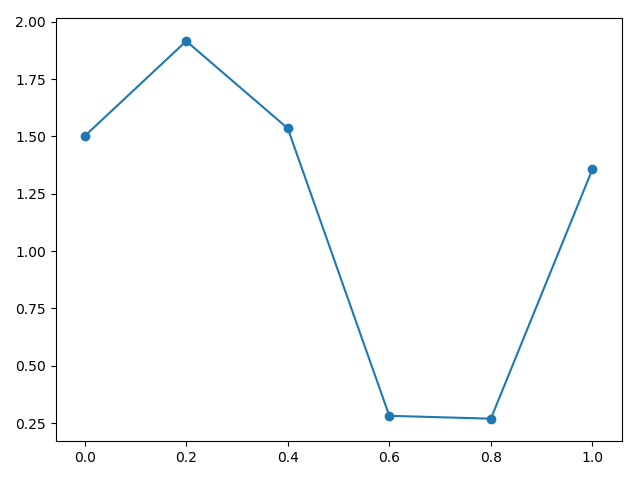
\includegraphics[width=7.5cm]{linear-interpolation}} \quad
  \subfigure[SBFIG:LINEAR2]{Bilinear interpolation}{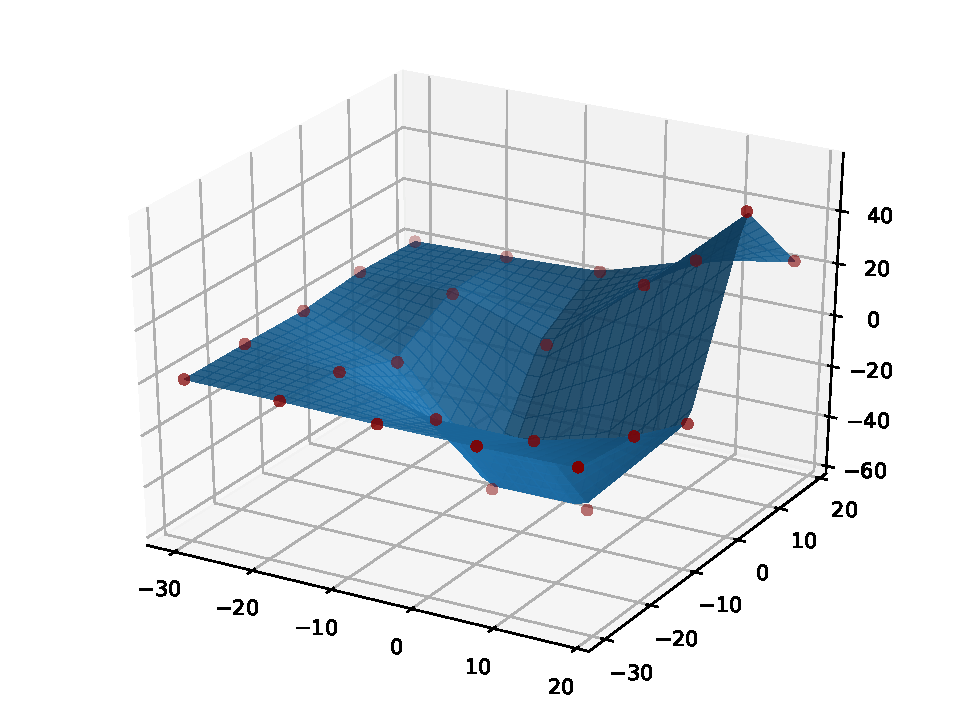
\includegraphics[width=7.5cm]{surface-bilinear}}
\end{figure}
